
\documentclass[a4paper,11pt]{article}%,twocolumn
%% packages

\usepackage{blindtext} % needed for creating dummy text passages
%\usepackage{ngerman} % needed for German default language
\usepackage{amsmath} % needed for command eqref
\usepackage{amssymb} % needed for math fonts
\usepackage[colorlinks=true,breaklinks]{hyperref} % needed for creating hyperlinks in the document, the option colorlinks=true gets rid of the awful boxes, breaklinks breaks lonkg links (list of figures), and ngerman sets everything for german as default hyperlinks language
\usepackage[hyphenbreaks]{breakurl} % ben�tigt f�r das Brechen von URLs in Literaturreferenzen, hyphenbreaks auch bei links, die �ber eine Seite gehen (mit hyphenation).
\usepackage{xcolor}
\definecolor{c1}{rgb}{0,0,1} % blue
\definecolor{c2}{rgb}{0,0.3,0.9} % light blue
\definecolor{c3}{rgb}{0.3,0,0.9} % red blue
\hypersetup{
    linkcolor={c1}, % internal links
    citecolor={c2}, % citations
    urlcolor={c3} % external links/urls
}
%\usepackage{cite} % needed for cite
\usepackage[square,authoryear]{natbib} % needed for cite and abbrvnat bibliography style
\usepackage[nottoc]{tocbibind} % needed for displaying bibliography and other in the table of contents
\usepackage{graphicx} % needed for \includegraphics 
\usepackage{longtable} % needed for long tables over pages
\usepackage{bigstrut} % needed for the command \bigstrut
\usepackage{enumerate} % needed for some options in enumerate
%\usepackage{todonotes} % needed for todos
\usepackage{makeidx} % needed for creating an index
\makeindex
\usepackage{gensymb}
\usepackage{url}
\usepackage{psfrag}
\usepackage{multirow}
\usepackage{subfigure}
%% page settings

\usepackage[top=20mm, bottom=20mm,left=15mm,right=15mm]{geometry} % needed for page border settings
\parindent=0mm % for space of first line of new text block
\sloppy % for writing with hyphenless justification (tries to)
\hyphenation{} % use hyphenation of tolerance parametershttp://www.jr-x.de/publikationen/latex/tipps/zeilenumbruch.html
\hyphenpenalty=10000
\exhyphenpenalty=10000
\usepackage{fancyhdr} % needed for head and foot options
%% my macros

%% Text fomats
\newcommand{\tbi}[1]{\textbf{\textit{#1}}}

%% Math fonts
\newcommand{\bbA}{\mathbb{A}}
\newcommand{\bbB}{\mathbb{B}}
\newcommand{\bbC}{\mathbb{C}}
\newcommand{\bbD}{\mathbb{D}}
\newcommand{\bbE}{\mathbb{E}}
\newcommand{\bbF}{\mathbb{F}}
\newcommand{\bbG}{\mathbb{G}}
\newcommand{\bbH}{\mathbb{H}}
\newcommand{\bbI}{\mathbb{I}}
\newcommand{\bbJ}{\mathbb{J}}
\newcommand{\bbK}{\mathbb{K}}
\newcommand{\bbL}{\mathbb{L}}
\newcommand{\bbM}{\mathbb{M}}
\newcommand{\bbN}{\mathbb{N}}
\newcommand{\bbO}{\mathbb{O}}
\newcommand{\bbP}{\mathbb{P}}
\newcommand{\bbQ}{\mathbb{Q}}
\newcommand{\bbR}{\mathbb{R}}
\newcommand{\bbS}{\mathbb{S}}
\newcommand{\bbT}{\mathbb{T}}
\newcommand{\bbU}{\mathbb{U}}
\newcommand{\bbV}{\mathbb{V}}
\newcommand{\bbW}{\mathbb{W}}
\newcommand{\bbX}{\mathbb{X}}
\newcommand{\bbY}{\mathbb{Y}}
\newcommand{\bbZ}{\mathbb{Z}}
\usepackage[ framed, numbered]{matlab-prettifier}%framed,%
\usepackage{listings}
\usepackage{physics}
\usepackage{pdfpages}
\usepackage[toc,page]{appendix}
\usepackage{float}
% for code
\usepackage{listings}
\usepackage{color}
\usepackage{pifont}

\usepackage{scalerel,xparse}
\NewDocumentCommand\emojismile{}{
    \scalerel*{
        
\includegraphics{./figures/emoji/u1F62C.png}
    }{X}
}


% Define colors
\definecolor{codegreen}{rgb}{0,0.6,0}
\definecolor{codegray}{rgb}{0.5,0.5,0.5}
\definecolor{codepurple}{rgb}{0.58,0,0.82}
\definecolor{backcolour}{rgb}{0.95,0.95,0.92}
% Setup the listings package
\lstset{
    backgroundcolor=\color{backcolour},   
    commentstyle=\color{codegreen},
    keywordstyle=\color{magenta},
    numberstyle=\tiny\color{codegray},
    stringstyle=\color{codepurple},
    basicstyle=\footnotesize,
    breakatwhitespace=false,         
    breaklines=true,                 
    captionpos=b,                    
    keepspaces=true,                 
    numbers=left,                    
    numbersep=5pt,                  
    showspaces=false,                
    showstringspaces=false,
    showtabs=false,                  
    tabsize=2
}



\begin{document}
\begin{titlepage}
\center % Center everything on the page

%-------------------------------------------------------------------------------------
%	HEADING SECTIONS
%------------------------------------------------------------------------------------
\textbf{\large Department of Electrical and Computer Engineering}\\[0.5cm]
\textbf{\Large University of Colorado at Boulder}\\[1cm]
\textbf{\large ECEN5823 - Low Power Embedded Design Techniques}\\[2cm]

\includegraphics[width=0.3\textwidth]{figures/cu}\\[2cm] 

	
%-------------------------------------------------------------------------------------
%	TITLE SECTION
%------------------------------------------------------------------------------------
\textbf{\Huge Spring 2024, ECEN 5823 }\\[0.2cm]

\textbf{\Large Course Project Report}\\[5cm]


%----------------------------------------------------------------------------------------
%	MEMBERS SECTION
%----------------------------------------------------------------------------------------


\vfill

\textbf{\large Submitted by}

{\large Parth Thakkar}\\[0.5cm]

%----------------------------------------------------------------------------------------
%	DATE SECTION
%----------------------------------------------------------------------------------------

\textbf{\large Submitted on}\\
\textbf{\Large \today} % Date, change the \today to a set date if you want to be precise

%----------------------------------------------------------------------------------------

\vfill % Fill the rest of the page with whitespace

\end{titlepage}

\pagebreak

\tableofcontents
\listoffigures
\listoftables
\vfill
\begin{center}
    \textbf{\textit{*PDF is clickable}}
\end{center}

\pagebreak

\section{Project Proposal}
\textbf{Team name:}\\
Low Self Esteem Team\\

\textbf{Student Name:}\\
Parth Rajeshkumar Thakkar\\
ParthRajeshkumar.Thakkar@colorado.edu\\

Anagha Aditya\\
Anagha.Aditya@colorado.edu\\

Akash Karoshi\\
Akash.Karoshi@colorado.edu\\


\section{Project Rationale and Goals}
For the ECEN 5833 Low Power Embedded System Design course, our team is developing an advanced mechanical keyboard called "The Insane Keyboard". This project aims to create a high-performance input device that combines ergonomic design, customization options, and some cool features.


\subsection{Project Rationale}
Our analysis of the mechanical keyboard market revealed several issues:
\begin{itemize}
    \item Ergonomic keyboards often lack additional features or are expensive
    \item Many feature-rich keyboards are wired, limiting mobility
    \item Affordable keyboards offer limited customization
    \item Few keyboards combine ergonomic design, wireless capability, programmable lighting, and smart functions
    \item Keyboards with displays or extra features often have poor power efficiency
\end{itemize}
\subsection{Project Goals}
We aim to create a mechanical keyboard with the following features:
\begin{itemize}
    \item Split ergonomic design to reduce physical strain
    \item Wireless connectivity using Bluetooth Low Energy.
    \item Programmable RGB lighting with addressable LEDs
    \item Hot-swappable key switches for easy customization
    \item Low-power E-ink display for additional information
    \item Multi-device compatibility
    \item Advanced power management techniques
    \item Environment temperature and pressure sensing.
    \item Real Time clock module for timer, stopwatch and time features.
    \item Potential energy harvesting from typing (Yet to be seen)
    \item Open-source firmware for extensive customization
    \item Cost-effective design for market accessibility
\end{itemize}

\subsection{Unique Features}
"The Insane Keyboard" has unique features like:
\begin{itemize}
    \item Integration of multiple desirable features in one device
    \item Optimized power management for extended use
    \item Potential energy harvesting from typing motions
    \item Open-source firmware for community-driven development
    \item Adaptable design for future upgrades
\end{itemize}

\subsection{Expected Outcomes}
Upon completion, this project could:
\begin{itemize}
    \item Improve ergonomics in daily computer use
    \item Advance keyboard power management and energy harvesting
    \item Foster a community of keyboard enthusiasts and developers
    \item Demonstrate practical applications of low-power embedded design
\end{itemize}

\section{Existing Products and Ideas from products}

% Placeholder for a diagram of the keyboard design
\begin{figure}[H]
    \centering
    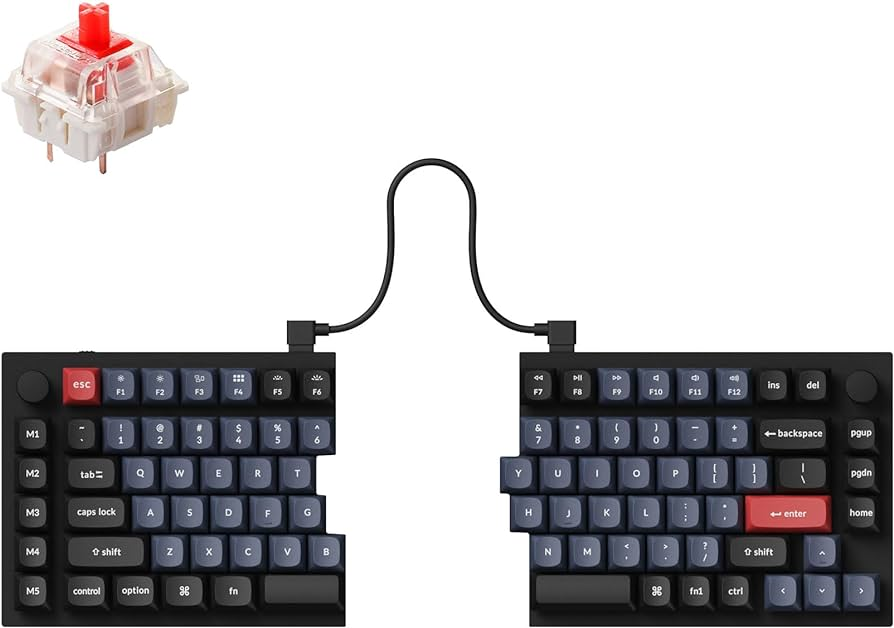
\includegraphics[scale=0.53]{figures/split_keyboard.jpg}
    \caption{Split Keyboard without display(Wired)}
    % Figure content to be added
\end{figure}
\vspace{0.2cm}
\begin{figure}[H]
    \centering
    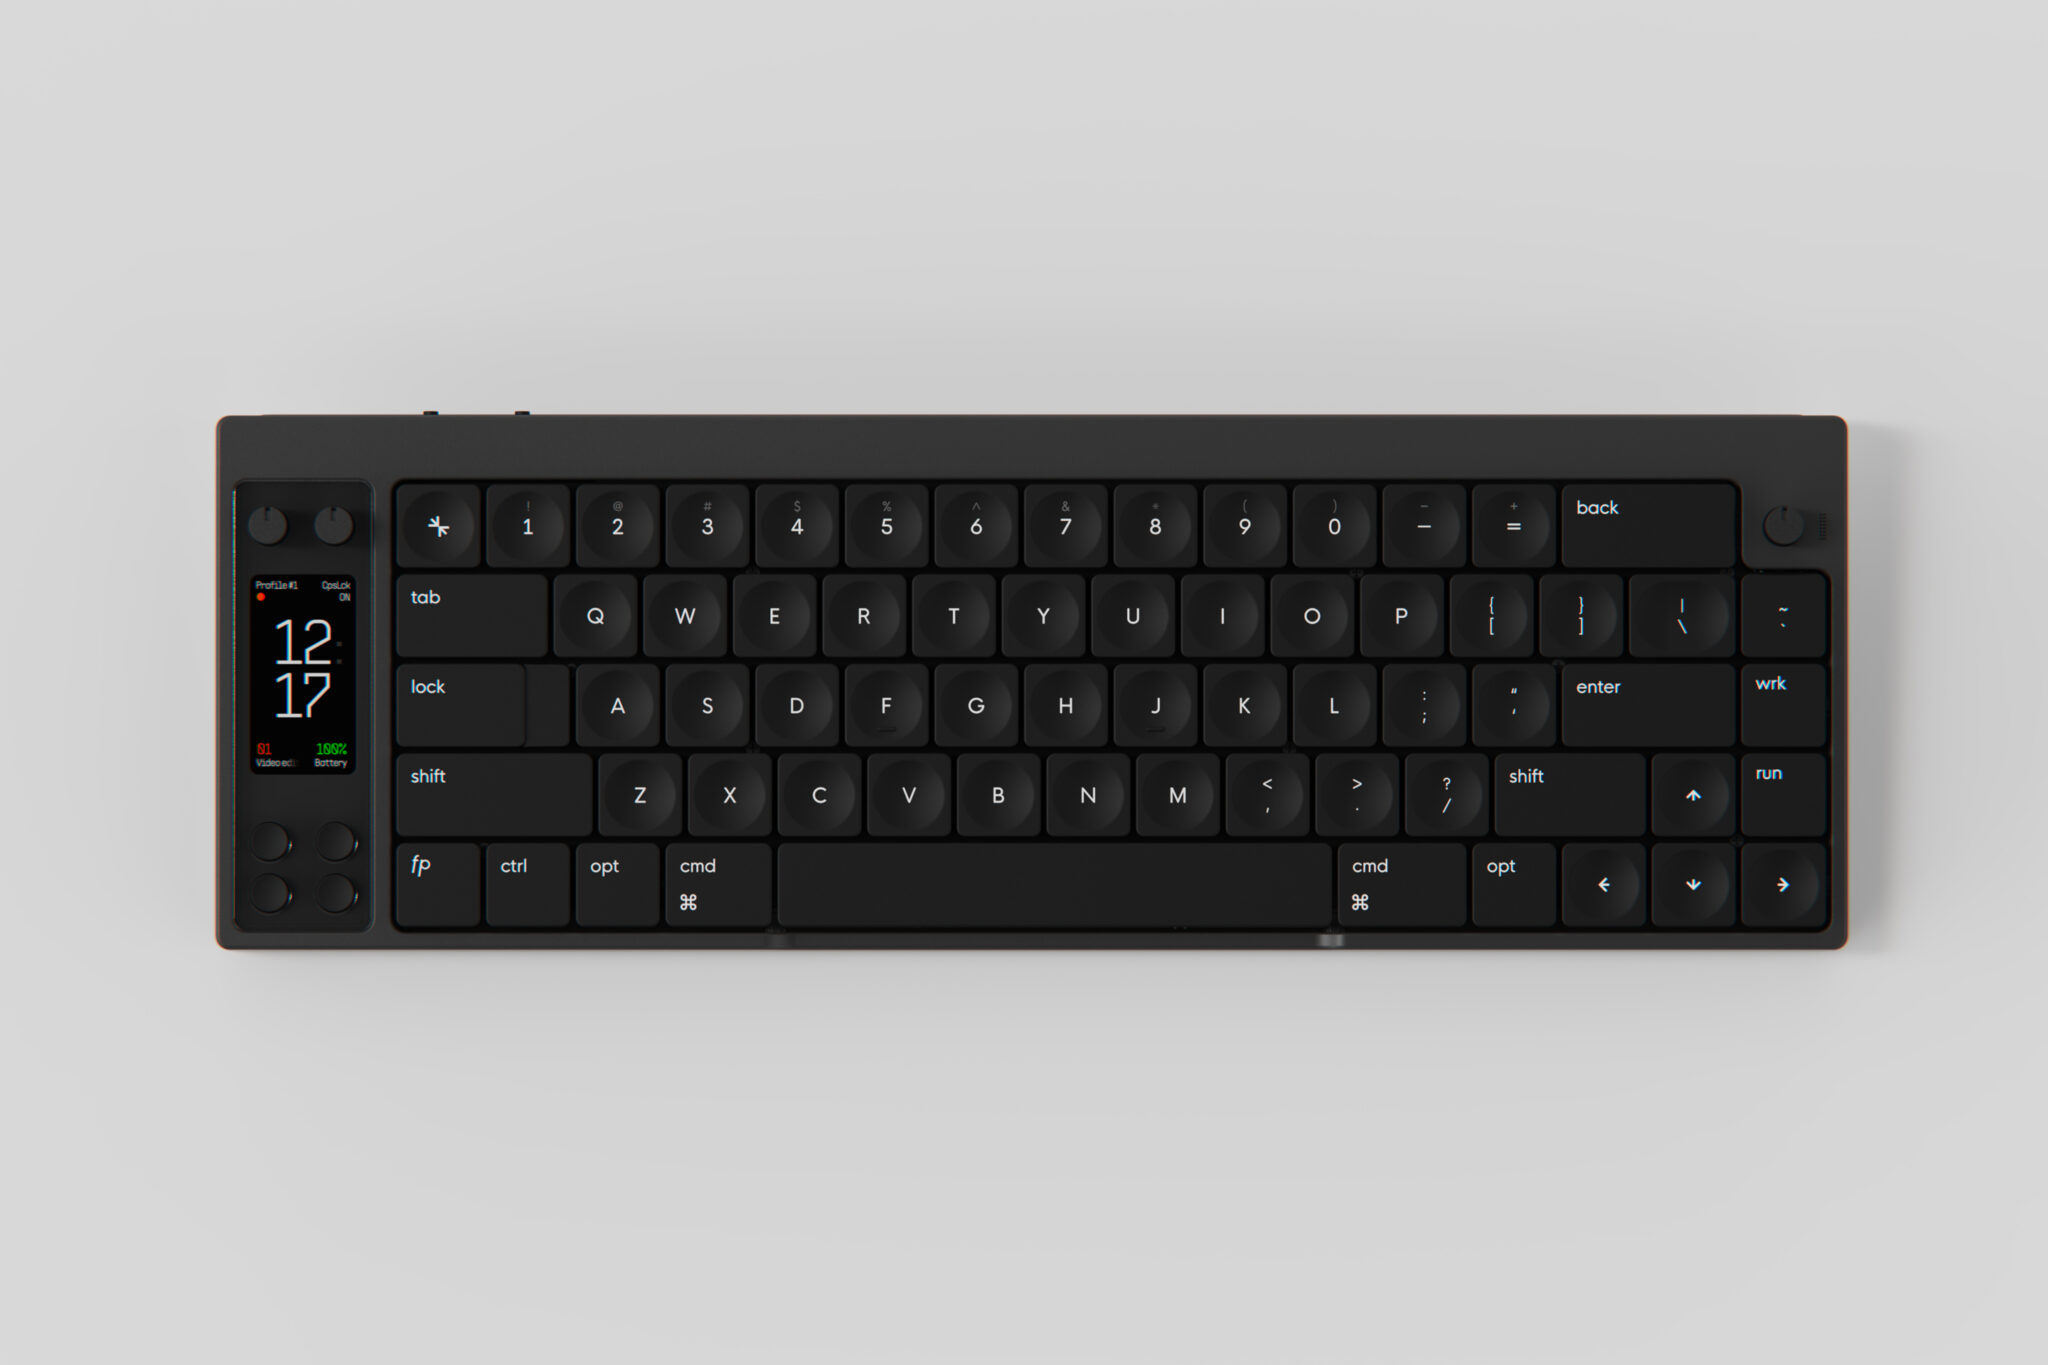
\includegraphics[scale=0.26]{figures/nomad.jpg}
    \caption{Keyboard which is expensive and have a Display}
    % Figure content to be added
\end{figure}
\vspace{0.2cm}

\begin{figure}[H]
    \centering
    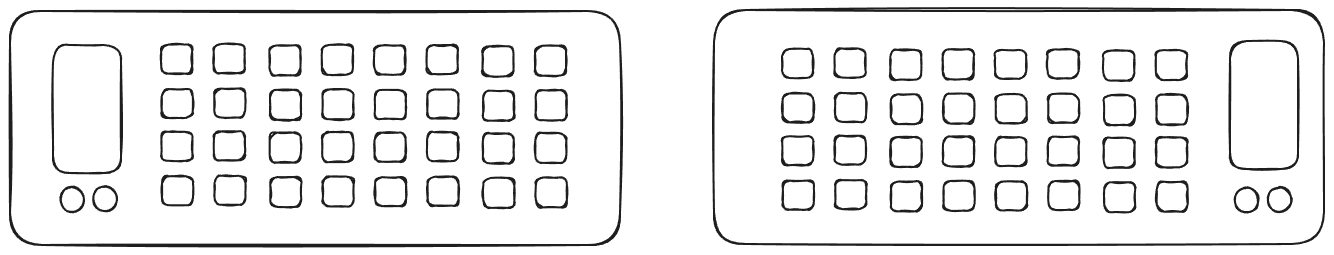
\includegraphics[scale=0.38]{figures/concept.png}
    \caption{Conceptual Design of The Insane Keyboard}
    % Figure content to be added
\end{figure}
\vspace{0.2cm}

\section{Project Timeline}

\begin{figure}[H]
    \centering
    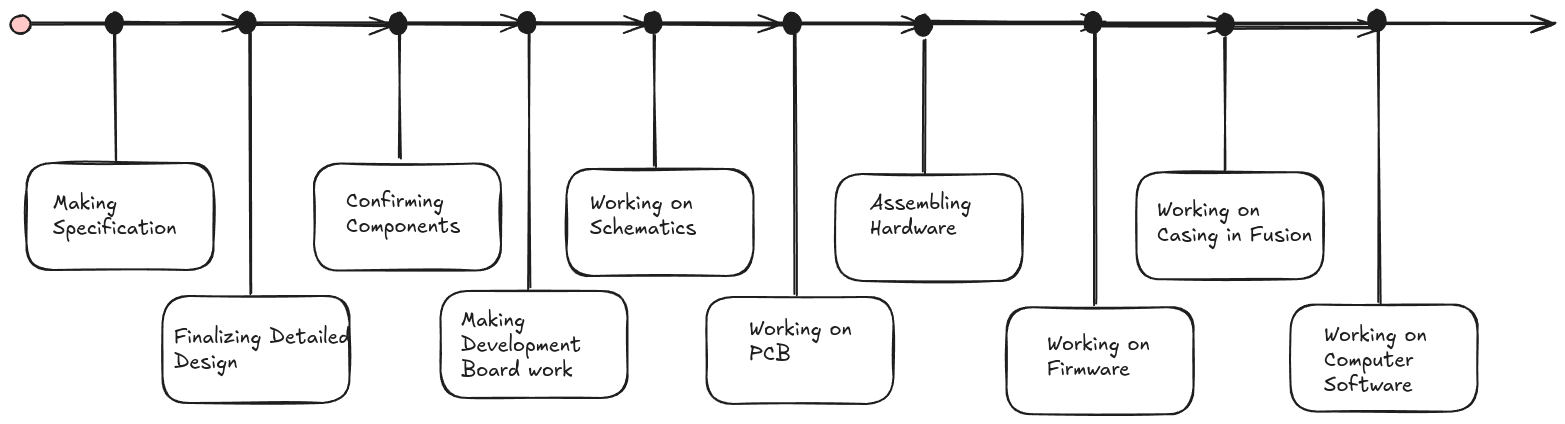
\includegraphics[scale=0.34]{figures/Timeline.png}
    \caption{Conceptual Design of The Insane Keyboard}
    % Figure content to be added
\end{figure}
\vspace{0.2cm}

\textbf{Kanban chart for project management, link for github :} \\
\href{https://github.com/users/parthishere/projects/2}{GITHUB Project}\\
\href{https://github.com/parthishere/Insane-Keyboard}{GITHUB Code link}
\begin{figure}[H]
    \centering
    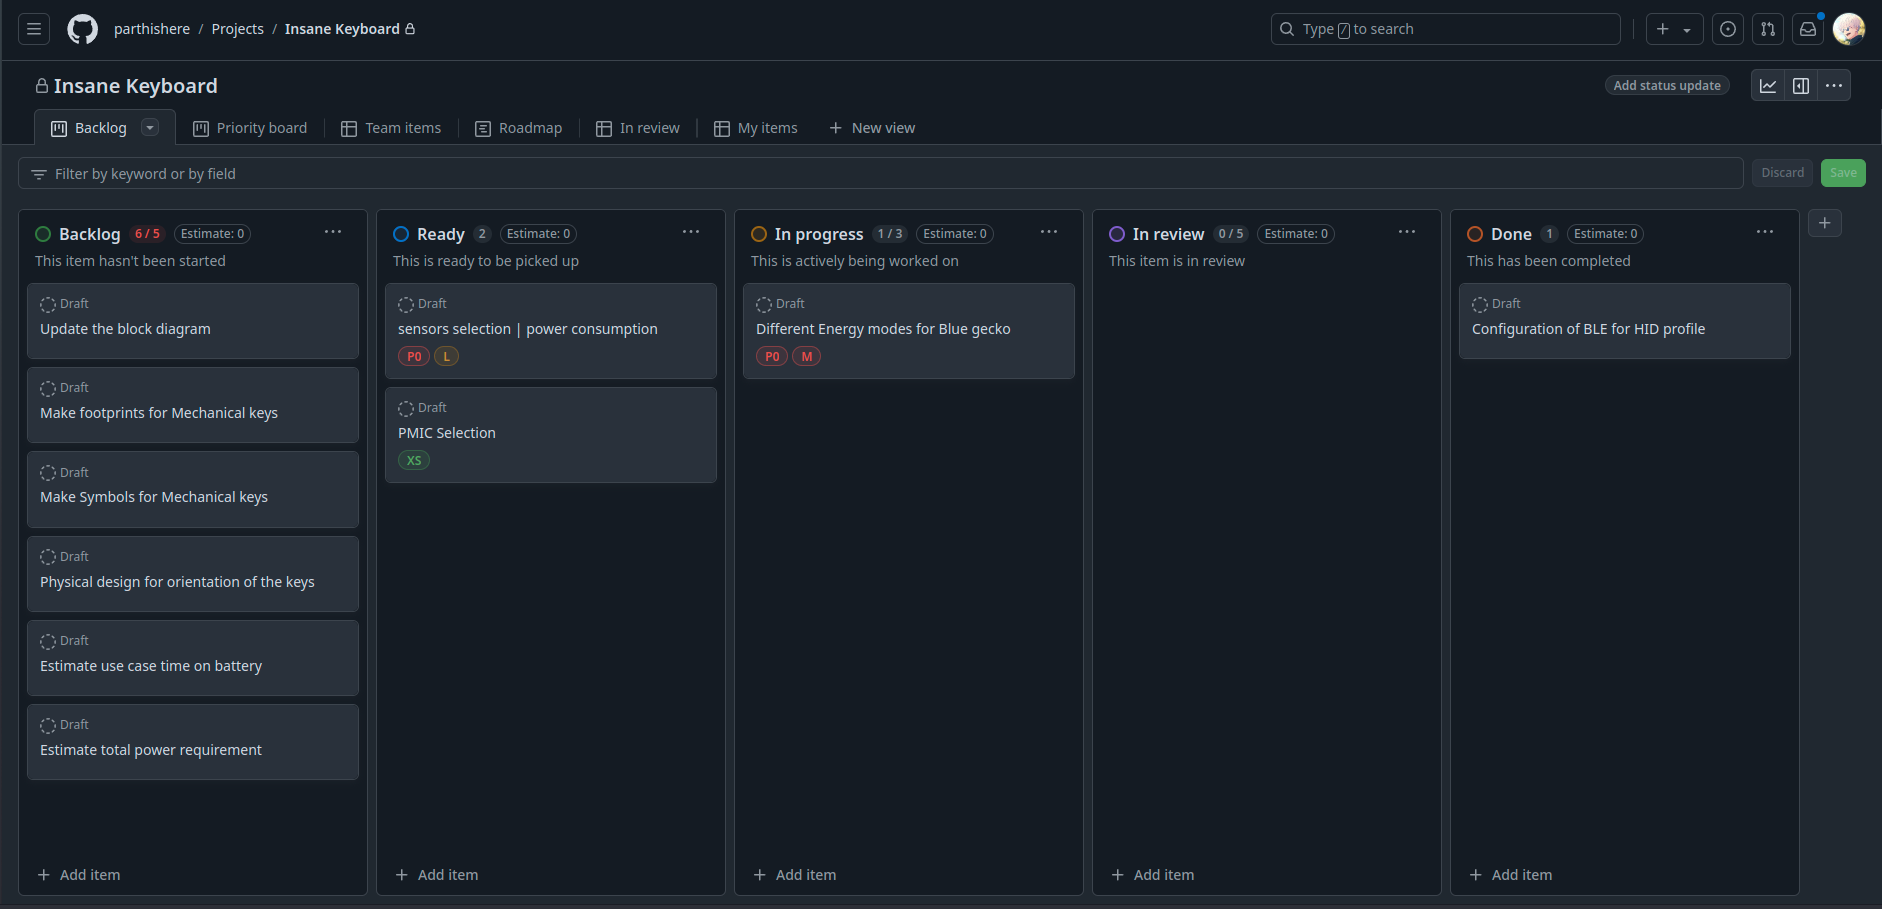
\includegraphics[scale=0.26]{figures/kanban.png}
    \caption{Kanban Board}
    % Figure content to be added
\end{figure}




\section{High Level Requirements}


\subsection{General Requirements}
\begin{itemize}
\item Two EFR32BG13 boards (one per module)
\item Should be Ergonomic
\item 75\% keyboard layout (TKL layout)
\item IO expander for each MCU
\item Temperature sensor
\item Pressure sensor
\item Real-Time Clock (RTC)
\item Connectivity to three host devices
\item Computer software for LED customization
\item Individually customizable LEDs
\item E-ink display on each module
\item Energy harvesting on each module
\item Charging circuit with Type-C connector
\item Charging indicator
\item Battery indicator
\item Minimum 6-key rollover
\item HID protocol communication between modules
\item Smart power states (active, idle, deep sleep)
\item RTOS: FreeRTOS (Yet to be decide)
\item PWM-based RGB LED control
\item Hot-swappable key switches
\item Time, date, battery status, current profile, custom graphics
\item Spotify integration for music control and now-playing information(yet to be seen)
\end{itemize}

\subsection{Components}
\begin{longtable}{|p{3cm}|p{2cm}|p{4cm}|p{2cm}|p{5cm}|}
    \hline
    \textbf{Component} & \textbf{Quantity} & \textbf{Function} & \textbf{Interface} & \textbf{URL} \\
    \hline
    EFR32BG13 & 2 & Microcontroller & - & \href{https://www.silabs.com/mcu/32-bit-microcontrollers/efm32pg23-series-2}{EFR32BG13 Series 1} \\
    \hline
    TCA6408A & 2 & IO Expander & I2C & \href{https://www.ti.com/lit/ds/symlink/tca6408a.pdf?HQS=dis-dk-null-digikeymode-dsf-pf-null-wwe&ts=1726372582102&ref_url=https%253A%252F%252Fwww.ti.com%252Fgeneral%252Fdocs%252Fsuppproductinfo.tsp%253FdistId%253D10%2526gotoUrl%253Dhttps%253A%252F%252Fwww.ti.com%252Flit%252Fgpn%252Ftca6408a}{TCA6408A Expander} \\
    \hline
    % TLC5947 & PWM Driver for LED & SPI & \href{https://www.ti.com/product/TLC5947}{TLC5947 Driver} \\
    % \hline
    % WS2815 & RGB LED (Individually Addressable) & - & - \\
    % \hline
    Waveshare E-ink Display & 1 &Display & SPI & \href{https://www.waveshare.com/1.54inch-e-Paper-Module.htm}{Waveshare E-ink display} \\
    \hline
    SI7021 & 1 &Temperature and Humidity Sensor & I2C & \href{https://www.silabs.com/documents/public/data-sheets/Si7021-A20.pdf}{SI7021 Sensor} \\
    \hline
    Schottky Diodes & 1 &Power Management & - & - \\
    \hline
    Gateron G Black Pro 2.0 & 68 & Key Switches & - & \href{https://www.amazon.com/Pre-lubed-Switches-Mechanical-Keyboard-Switches/dp/B0BH1BZ787/ref=sr_1_3?dib=eyJ2IjoiMSJ9.Znh8d8tPJSWiImgJJpmm-QaZyTnVNKNJ_kJO8F-VsBufwkYWPE22tiWw0cJ-akUZp0mCPOwwRMy-WRHf2F9g0Dvac17T6EuiT9uTNjLg1UvHb6A5IJ-fiwz_bSpWSV10Awtk7U7hSs_WaEn9z6pZjk1Ua2gutyyzVToMb1ntQ8q7pWGvrrvOeiEwpwiIWQBDviCxxIlD7fl0UUH_JJ9kOp_C_17x0PXvYOHWw8FYhn8.gS8VP-4QbafCra1X6UlUj1E0eMfB4ogbHozN37MjJ1Q&dib_tag=se&keywords=gateron%2Bblack&qid=1725254581&sr=8-3&th=1}{Gateron G black Pro 2.0} \\
    \hline
    Mechanical Key hotswap & 68 &Hot swap  & - & \href{https://www.amazon.com/dp/B0CZ79GGDF?ref=ppx_yo2ov_dt_b_fed_asin_title}{Gateron G black Pro 2.0} \\
    \hline
    Cherry MX Key Caps & 68 &Key Caps & - & \href{https://www.aliexpress.com/item/3256801599125271.html?spm=a2g0o.order_list.order_list_main.5.43b918023cg2lz}{Cherry MX Key Caps} \\
    \hline
    Rotary Encoders & 2 &Input Device & - & \href{https://www.adafruit.com/product/377}{Rotary Encoders} \\
    \hline
    \caption{Component List for The Insane Keyboard}
    \label{tab:components}
    \end{longtable}
    
\section{Keyboard Layout and Design}

\subsection{Main Board Key Layout}
\begin{center}
\begin{tabular}{|c|c|c|c|c|c|c|}
\hline
\multicolumn{7}{|c|}{\textbf{Function Row}} \\ \hline
\begin{tabular}[c]{@{}c@{}}ESC\ $\sim$ `{}\end{tabular} &
\begin{tabular}[c]{@{}c@{}}F1\ 1 !\end{tabular} &
\begin{tabular}[c]{@{}c@{}}F2\ 2 @\end{tabular} &
\begin{tabular}[c]{@{}c@{}}F3\ 3 \#\end{tabular} &
\begin{tabular}[c]{@{}c@{}}F4\ 4 \$\end{tabular} &
\begin{tabular}[c]{@{}c@{}}F5\ 5 \%\end{tabular} &
\begin{tabular}[c]{@{}c@{}}F6\ 6 \^{}\end{tabular} \\
\hline
\multicolumn{7}{|c|}{\textbf{QWERTY Row}} \\
\hline
TAB & Q & W & E & R & T &\\
\hline
\multicolumn{7}{|c|}{\textbf{Home Row}} \\
\hline
CAPS & A & S & D & F & G & \\
\hline
\multicolumn{7}{|c|}{\textbf{Bottom Row}} \\
\hline
SHIFT & Z & X & C & V & B & \\
\hline
\multicolumn{7}{|c|}{\textbf{Modifier Row}} \\
\hline
CTRL & OPT & WIN/MAC & ALT & \multicolumn{3}{c|}{SPACE} \\
\hline
\end{tabular}
\end{center}
\textbf{Additional Inputs:}
\begin{itemize}
\item 2 × Rotary Encoders (Knobs)
\item 3 × Extra Buttons
\end{itemize}
\textbf{Additional Components}
\begin{itemize}
    \item E-Ink display
    \item Battery
    \item Battery Charging and Power Management Unit \textcolor{yellow}{(Not in Secondary module)}
    \item Tempurature Sensor \textcolor{yellow}{(Not in Secondary module)}
    \item Real time Clock \textcolor{yellow}{(Not in Secondary module)}
\end{itemize}

\subsection{Secondary Module Key Layout}
\begin{center}
\begin{tabular}{|c|c|c|c|c|c|c|c|}
\hline
\multicolumn{8}{|c|}{\textbf{Function Row}} \\
\hline
F7 & F8 & F9 & F10 & F11 & F12 & BKSP & HOME \\
\hline
\multicolumn{8}{|c|}{\textbf{QWERTY Row}} \\
\hline
Y & U & I & P & \{[ & \}] & |$\backslash$  & DEL \\
\hline
\multicolumn{8}{|c|}{\textbf{Home Row}} \\
\hline
H & J & K & L & \begin{tabular}[c]{@{}c@{}}; :\end{tabular} & \begin{tabular}[c]{@{}c@{}}" '\end{tabular} & ENTER & PGUP \\
\hline
\multicolumn{8}{|c|}{\textbf{Bottom Row}} \\
\hline
N & M & \begin{tabular}[c]{@{}c@{}}, <\end{tabular} & \begin{tabular}[c]{@{}c@{}}. >\end{tabular} & \begin{tabular}[c]{@{}c@{}}/ ?\end{tabular} & SHIFT & ↑ & PGDN \\
\hline
\multicolumn{8}{|c|}{\textbf{Modifier Row}} \\
\hline
& SPACE & ALT/MAC & FN & CTRL & ← & ↓ & → \\
\hline
\end{tabular}
\end{center}
\textbf{Additional Inputs:}
\begin{itemize}
\item 2 × Rotary Encoders (Knobs)
\item 3 × Extra Buttons
\end{itemize}
\textbf{Additional Components:}
\begin{itemize}
    \item E-Ink display
    \item Battery
    \item Power Management Unit
\end{itemize}

\section{Technical Considerations}


\subsection{Functional hardware block diagram}



\begin{figure}[H]
    \centering
    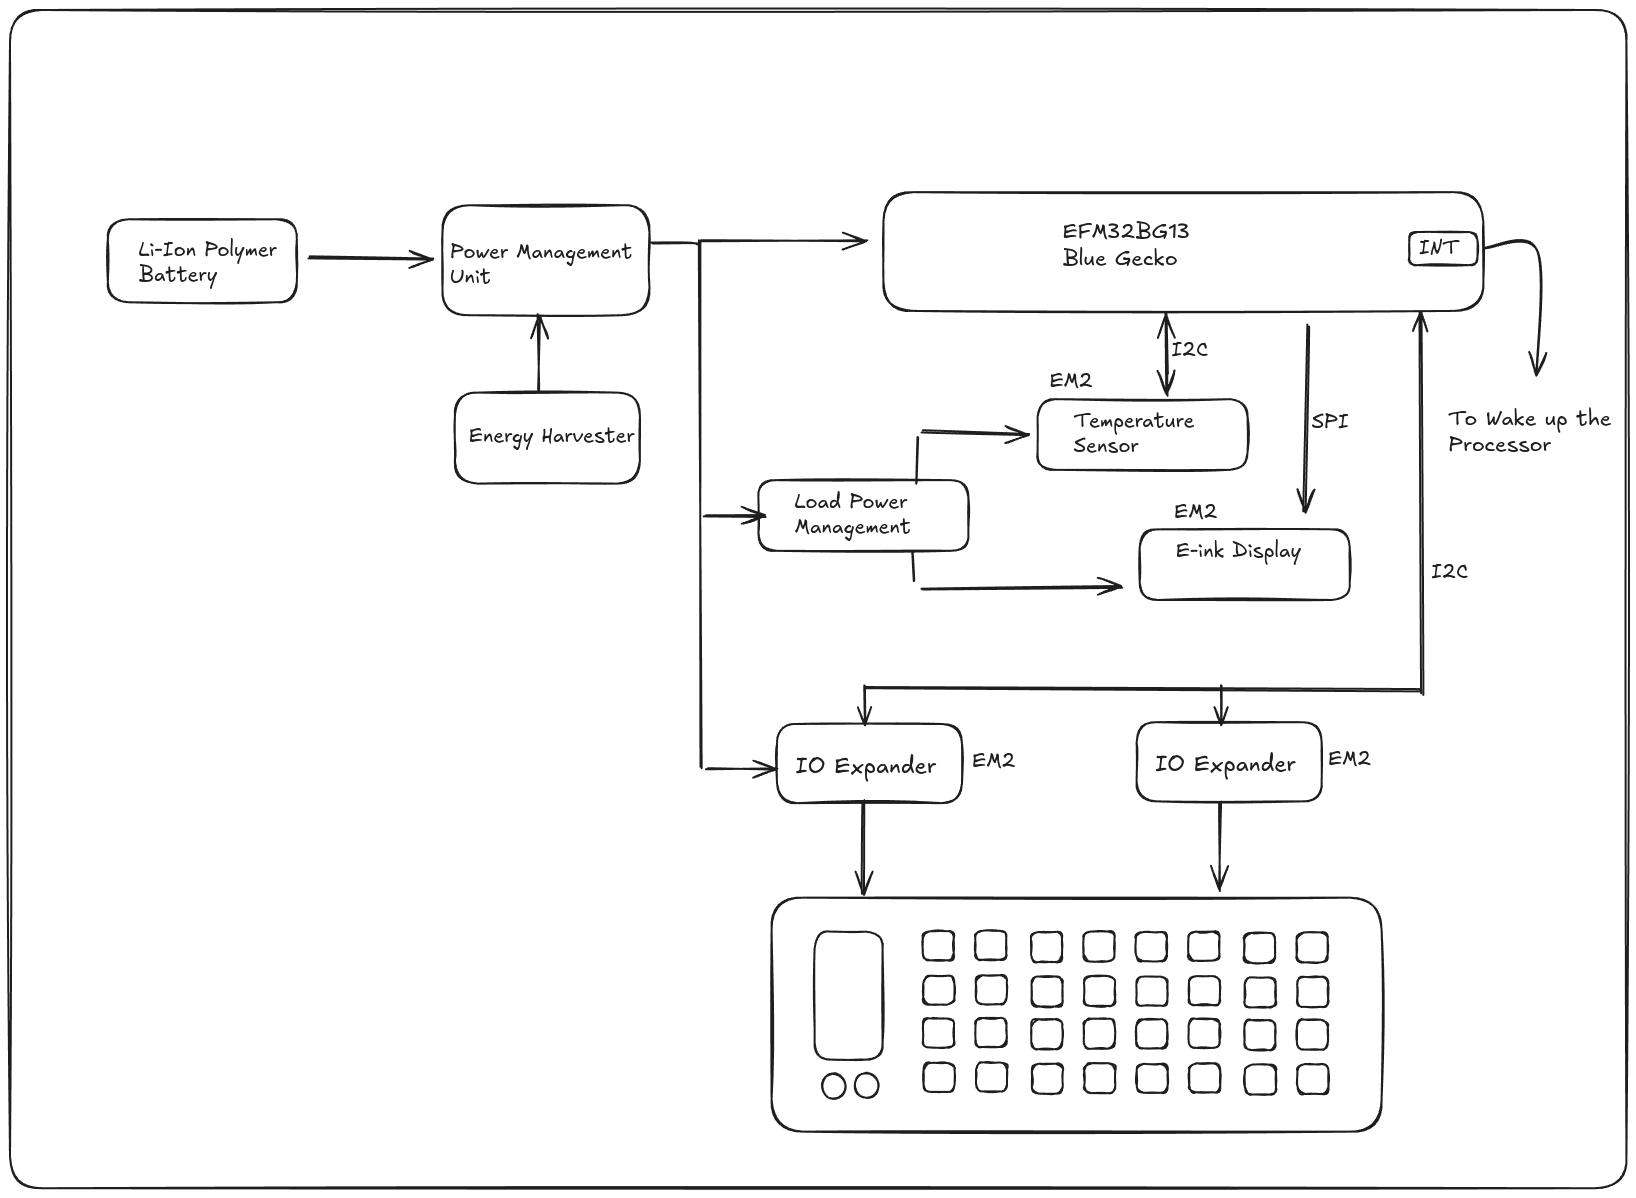
\includegraphics[scale=0.32]{figures/blockdiagram.png}
    \caption{Hardware block diagram}
    % Figure content to be added
\end{figure}
\vspace{0.2cm}


\textbf{0-Key Rollover (Normal Matrix)}
\begin{figure}[H]
	\centering
	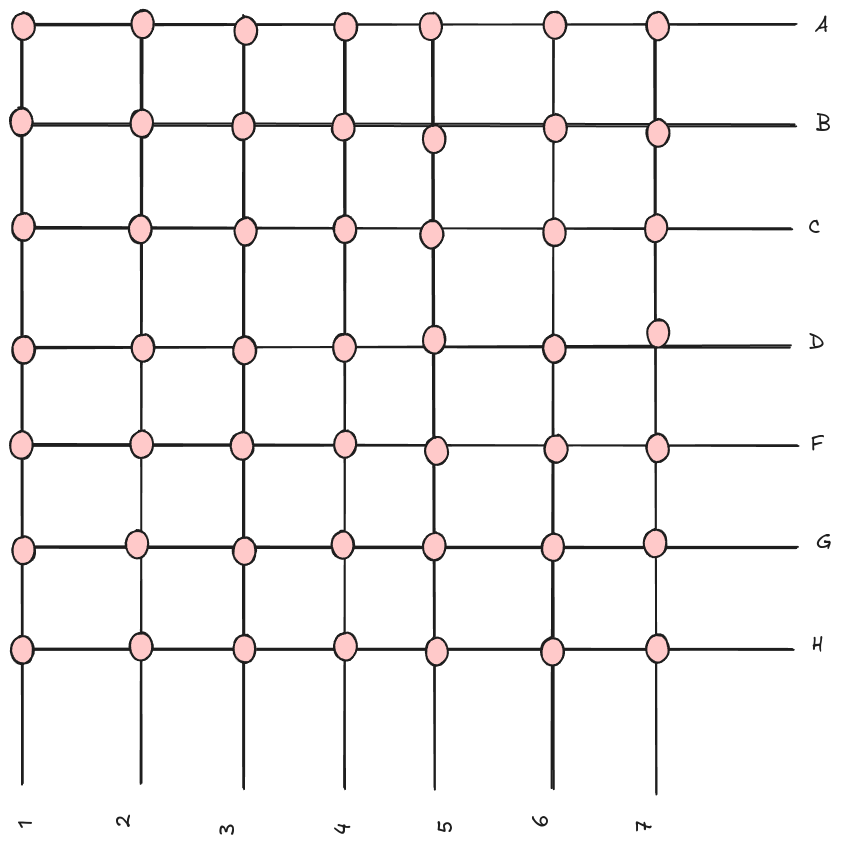
\includegraphics[scale=0.6]{figures/NRO.png}
	\caption{Normal Matrix for no key roll over}
\end{figure}
\begin{figure}[H]
	\centering
	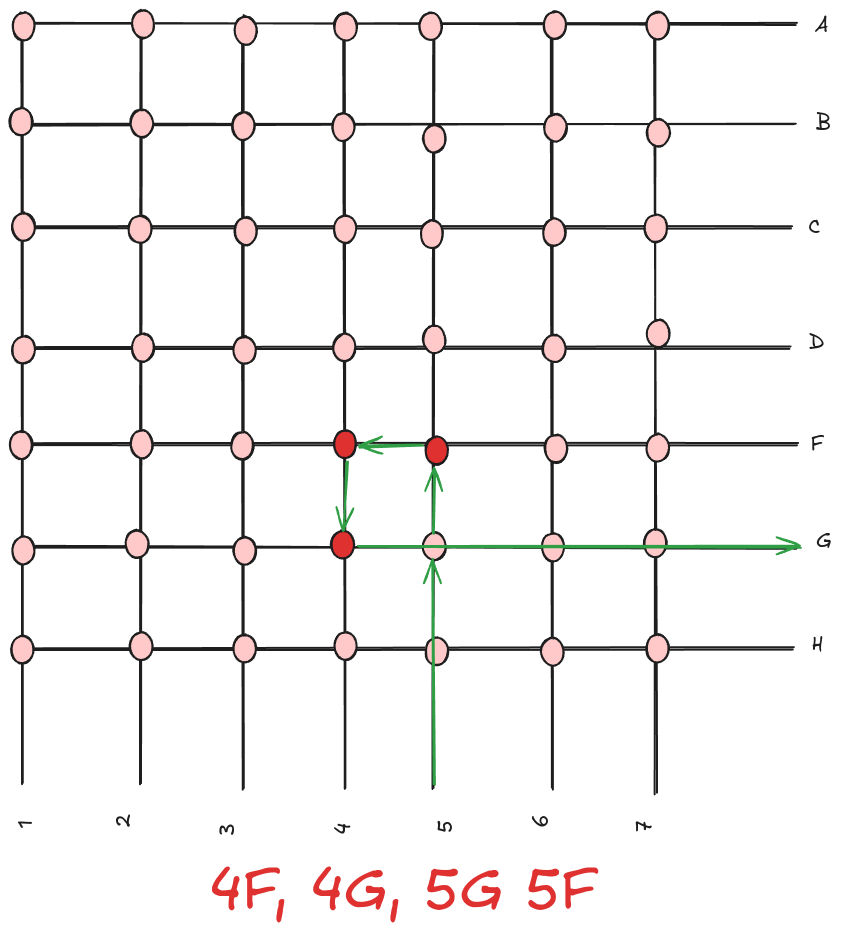
\includegraphics[scale=0.6]{figures/nkr-EX.png}
	\caption{Decoding wrong button press}
\end{figure}

\textbf{N-Key Rollover feature with Diodes}
\begin{figure}[H]
    \centering
    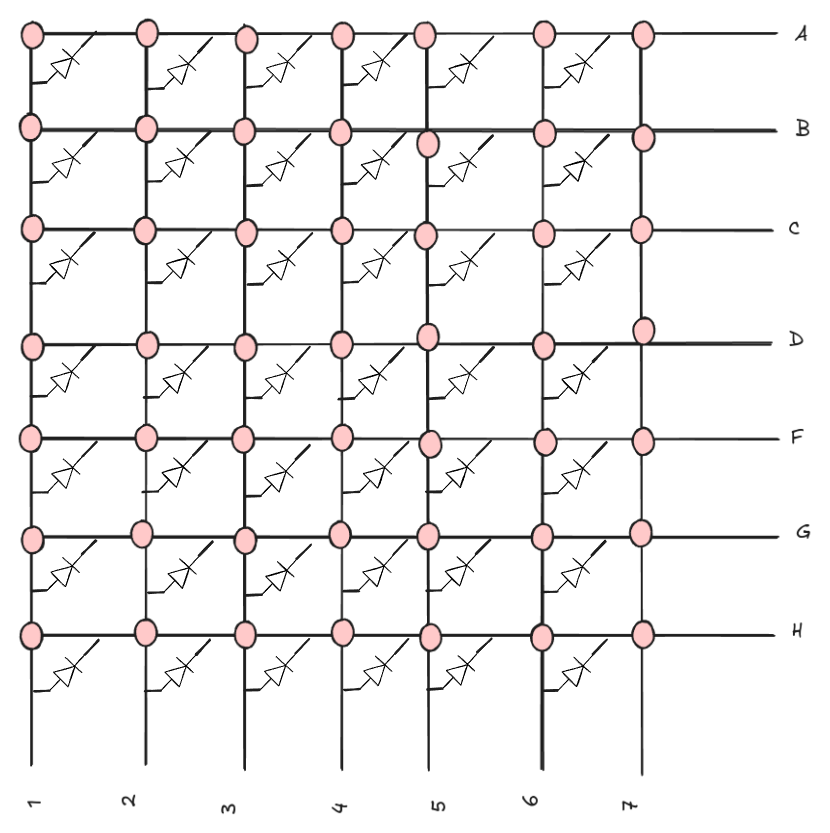
\includegraphics[scale=0.6]{figures/NKRO.png}
    \caption{N-Key Rollover}
\end{figure}

\begin{figure}[H]
	\centering
	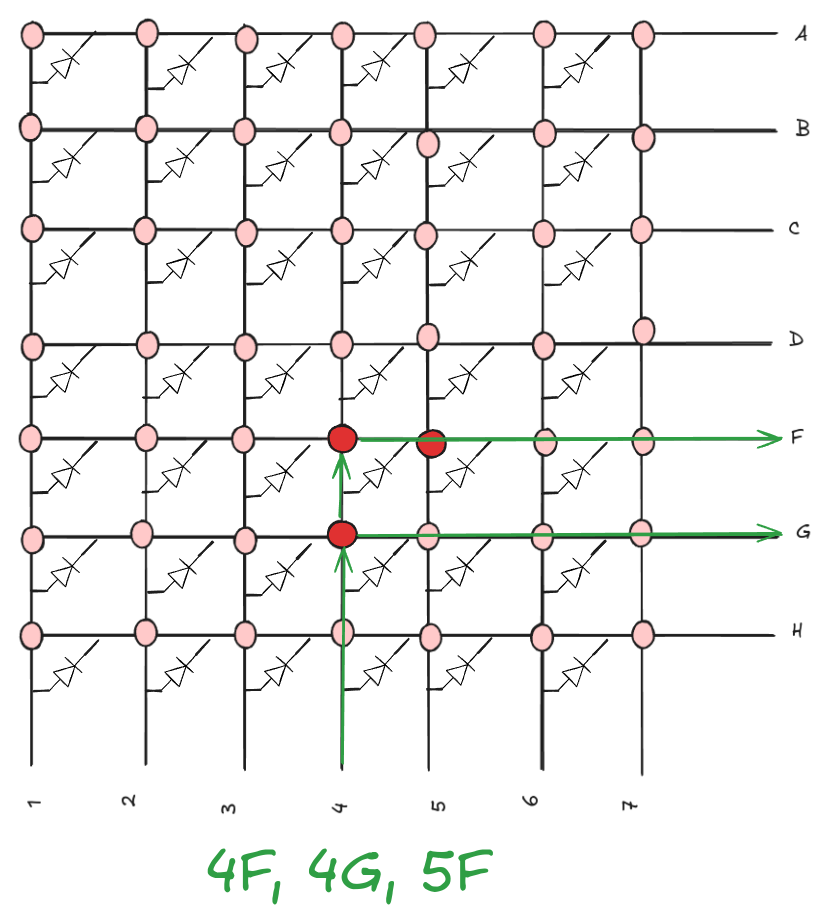
\includegraphics[scale=0.6]{figures/NKRO-EX.png}
	\caption{Multiple keys pressed}
\end{figure}




The keyboard uses a matrix layout, which is an efficient way to manage multiple key inputs with fewer microcontroller pins. In the images, we see an 8x7 matrix (rows A-H, columns 1-7).\\
Scanning Process:\\

The microcontroller scans this matrix by activating one column at a time and reading the state of all rows.
When a key is pressed, it connects a row and column, which the microcontroller detects.\\


\textbf{Ghosting and Its Prevention:}

Ghosting is a problem in simple matrix designs where pressing multiple keys can lead to false key registrations.
Example (Image 1):\\

If keys at 4F, 4G, and 5F are pressed simultaneously, the matrix might also falsely register 5G.\\

\textbf{Solution (Images 2 and 3):}

Diodes are added to each key switch.
These diodes allow current to flow in only one direction, preventing the "phantom" current paths that cause ghosting.
With diodes, when 4F, 4G, and 5F are pressed, 5G is not falsely registered.\\


\textbf{N-Key Rollover (NKRO):}

NKRO allows the keyboard to correctly register any number of simultaneous key presses.\\
Implementation:\\

Each key gets its own diode, ensuring independent registration.
The microcontroller scans the entire matrix rapidly, detecting all pressed keys without conflicts.\\


\textbf{Hardware Components:}

\textbf{Central Microcontroller:}

EFM32BG13 Blue Gecko: This MCU manages all keyboard functions and interfaces with other components.\\

\textbf{Sensors:}

TMP117: Measures temperature, humidity, and pressure, potentially for environmental adaptation or user information.\\
DS3231 RTC Module: Provides accurate timekeeping, useful for time-based functions or logging.\\

\textbf{Display}:

E-Ink Display (800x600, 4.3inch): Offers a low-power way to show keyboard status, settings, or other information.\\

\textbf{Expansion:}

MCP23017 IO Expander: Increases the number of available pins for the key matrix, allowing for more keys or other inputs.\\

\textbf{Power Management:}

Power Management Unit: Manages power distribution and consumption.\\
Li-Ion Polymer Battery: Provides portable power.\\
Energy Harvester: Potentially extends battery life by capturing ambient energy.\\

\textbf{Key Switches and Caps:}

Gateron G Black Pro 2.0 switches: Known for smooth linear action.
Cherry MX key caps: Industry-standard keycaps for customization.\\

\textbf{Additional Inputs:}

Rotary encoders: Provide alternative input methods, possibly for volume control or menu navigation.\\


\textbf{PCB Design:}

4-layer PCB: Allows for more complex routing and better signal integrity.\\
Two versions:\\

Main Module with  all sensors and charging capabilities.\\
Simplified Secondary Module without temperature, humidity, RTC, and LiPo charger.\\


\section{Wireless Communication and Software Architecture}
\subsection{Wireless Communication Details}


\begin{table}[H]
    \centering
    
    \begin{tabular}{|p{2.5cm}|p{2cm}|p{2cm}|p{1.2cm}|p{6cm}|}
    \hline
    \textbf{Char} & \textbf{Properties} & \textbf{Data Type} & \textbf{Length} & \textbf{Description} \\
    \hline
    Keyboard Input Report & Read, Notify & Uint8Array & 8 bytes & 
    \begin{itemize}
        \item Byte 0: Modifier keys
        \item Byte 1: Reserved
        \item Bytes 2-7: Pressed key codes
    \end{itemize} \\
    \hline
    Keyboard Output Report & Read, Write & Uint8Array & 1 byte & 
    \begin{itemize}
        \item Bit 0: Num Lock
        \item Bit 1: Caps Lock
        \item Bit 2: Scroll Lock
        \item Bit 3: Compose
        \item Bit 4: Kana
        \item Bits 5-7: Reserved
    \end{itemize} \\
    \hline
    Protocol Mode & Read, Write & Uint8 & 1 byte & 
    \begin{itemize}
        \item 0x00: Boot Protocol
        \item 0x01: Report Protocol
    \end{itemize} \\
    \hline
    HID Information & Read & Uint16, Uint8, Uint8 & 4 bytes & 
    \begin{itemize}
        \item Bytes 0-1: bcdHID
        \item Byte 2: bCountryCode
        \item Byte 3: Flags
    \end{itemize} \\
    \hline
    HID Control Point & Write & Uint8 & 1 byte & 
    \begin{itemize}
        \item 0x00: Suspend
        \item 0x01: Exit Suspend
    \end{itemize} \\
    \hline
    Report Map & Read & Uint8Array & Variable & Defines the format of Input and Output reports \\
    \hline
    \end{tabular}
    \caption{HID Profile Characteristics for Keyboard}
    \end{table}


\pagebreak
\subsection{Functional software block diagram}
\begin{figure}[H]
    \centering
    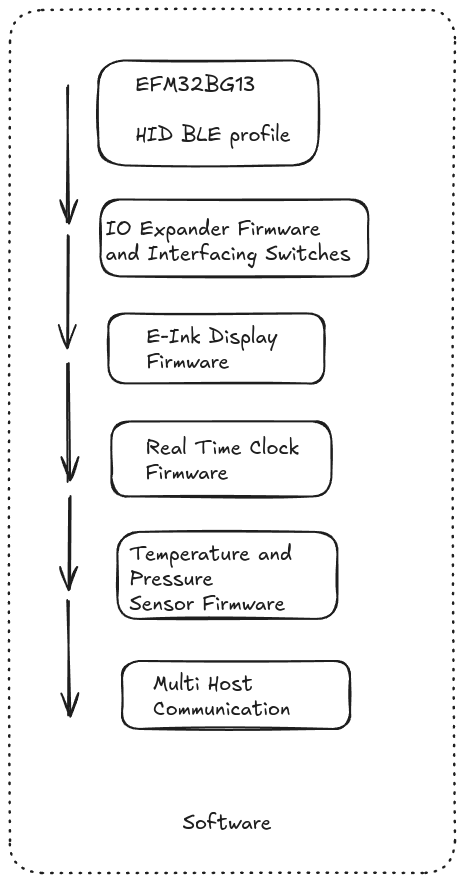
\includegraphics[scale=0.44]{figures/software_diagram.png}
    \caption{Software block diagram}
    % Figure content to be added
\end{figure}
\vspace{0.2cm}


\section{Challenges and Considerations}
\begin{itemize}
\item Managing state machines with complex software like e-ink display drivers
\item Integrating drivers with BLE firmware
\item Implementing RTC driver and temperature control driver
\item Ensuring reliable wireless connectivity
\item Implementing multi-host communication and switching
\item Developing HID profile in BLE stack
\item Implementing anti-ghosting techniques
\item Optimizing keyboard scan rate for low latency
\item Achieving N-key rollover or 6-key rollover
\end{itemize}



% \subsubsection{User interface}

% Buttons:
% \begin{enumerate}
%     \item PB1 Button (Bonding Initiation):
%           \begin{itemize}
%               \item The PB1 button is used to initiate the bonding process between the server and the client.
%               \item When the user presses the PB1 button on the server, it triggers the bonding request to the client.
%           \end{itemize}
%     \item PB0 Button (Bonding Confirmation):
%           \begin{itemize}
%               \item The PB0 button is used to confirm the bonding process on the client side
%               \item After the server/client initiates the bonding request, the client receives a notification.
%           \end{itemize}
%     \item The servo motor is used to provide a physical indication of the authentication status.
%           \begin{itemize}
%               \item If the received data matches the predefined values for a valid authentication, the servo motor is activated.
%           \end{itemize}
%     \item LED (Light-Emitting Diode):
%           \begin{itemize}
%               \item After the client processes the received RFID data and encoder value, it determines the authentication result.
%                     If the authentication is successful, the LED is turned on
%           \end{itemize}
%     \item The LCD is used to display detailed information and messages to the user.
%           \begin{itemize}
%               \item It can show the current status of the system, such as "Ready for Authentication," "Bonding in Progress," or "Authentication Successful."
%               \item The LCD can also display the received RFID data and encoder value for reference or debugging purposes.
%               \item In case of an authentication failure, the LCD can display an appropriate error message, such as "Wrong Card or Encoder Value."
%           \end{itemize}
% \end{enumerate}


% Interaction Flow:
% \begin{enumerate}
%     \item The user initiates the bonding process by pressing the PB1 button on the client.
%     \item The client sends a bonding request to the client, which is indicated on the LCD.
%     \item The user confirms the bonding by pressing the PB0 button on the server.
%     \item Once the bonding is established, the user can proceed with the authentication process.
%     \item The user presents the RFID card to the reader and adjusts the rotary encoder to the correct value.
%     \item The server detects the RFID card, reads the data, and sends it along with the encoder value to the client.
%     \item The client receives the data, processes it, and determines the authentication result.
%     \item If the authentication is successful, the LCD displays a success message, the LED turns on, and the servo motor performs a predefined movement.
%     \item If the authentication fails, the LCD displays an error message, the LED remains off, and the servo motor does not activate.
%     \item The user can retry the authentication process or take appropriate actions based on the feedback provided by the LCD, LED, and servo motor.
% \end{enumerate}




% \subsubsection{Subsystem}

% \begin{enumerate}
%     \item The RFID subsystem consists of an MFRC522 RFID reader module that reads RFID tag data when a tag is presented. It communicates with the server microcontroller using SPI interface and generates an interrupt to wake up the server from sleep mode when a tag is detected.

%     \item The Rotary Encoder Subsystem (hardware) captures user input by measuring the rotation and direction of the encoder. It generates an interrupt to wake up the server from sleep mode when rotated and provides values from -255 to 255 for authentication purposes.

%     \item The BLE Communication Subsystem (software) uses Silicon Labs EFR32BG13 Gecko Boards to securely connect between the server and client. It establishes a secure connection using bonding and encryption, and utilizes the Object Transfer Service (OTS) for transmitting RFID tag data. A custom Rotary Encoder Service is used for transmitting rotary encoder values.

%     \item The Data Compression Subsystem (software) compresses the RFID tag data and rotary encoder values before transmission. It reduces data sent over BLE while optimizing bandwidth and power consumption. Decompression is done on the receiving side to determine authentication status based on comparison results.
% \end{enumerate}

% % \begin{figure}[H]
% % 	\centering
% % 	\includegraphics[scale=0.42]{figures/subsystem.png}
% % 	\caption{User Interface}
% % 	\label{idealbpfilter}
% % \end{figure}


% \subsubsection{Test Plan}




% \textbf{GitHub repository URL:} \href{https://github.com/CU-ECEN-5823/ecen5823-courseproject-parthishere}{https://github.com/CU-ECEN-5823/ecen5823-courseproject-parthishere}



% \subsection{Challenges}

% One of the major challenges I encountered during the development process was the integration of the display and the RFID module. Despite having functional drivers for both components individually, combining them proved to be a complex task.\\

% The issue manifests when I initialize the display. As soon as the display is initialized, the RFID module stops responding and fails to read any RFID cards. This behavior suggests a potential conflict between the display and the RFID module, likely related to the SPI driver.\\

% I extensively investigated the problem and tried various approaches to resolve it. One of my initial attempts involved setting the chip select line high to deselect the RFID module when communicating with the display. However, even with this modification, the RFID module remained unresponsive, consistently returning a value of 0xFF when attempting to read any register.\\

% To further troubleshoot the issue, I explored the possibility of explicitly disabling the \texttt{sensor\_enable} pin, which controls the power supply to the display. By toggling this pin, I aimed to isolate the display and prevent any interference with the RFID module. Unfortunately, this approach did not yield the desired results, and the RFID module continued to exhibit the same unresponsive behavior.\\

% The complexity of the problem is compounded by the fact that the display driver is already implemented in the provided API, and modifying it is not a viable option. This limitation leads me to make certain assumptions about the API's functionality. One possibility is that the API does not properly handle the chip select line, as there is no explicit mention of it in the project configuration or generated files. It is unclear whether the chip select line is unused, not configured, held high by software, or managed internally by the API without being exposed in the configuration interface.\\

% To overcome this challenge, I am considering two potential solutions. The first approach involves explicitly disabling the \texttt{sensor\_enable} pin, deselecting the display's slave select line, and enabling the slave select line of the RFID module's SPI interface. By carefully managing these control signals, I aim to establish a clear separation between the display and the RFID module, preventing any conflicts during communication.\\

% The second approach entails modifying the USART pins used for the SPI interface. By using a different set of USART pins for the RFID module, such as USART2, I can avoid any clashes with the display's SPI interface. This solution would require reconfiguring the SPI driver and ensuring that the new pin assignments are compatible with the overall system design.\\

% Resolving the integration challenge between the display and the RFID module is a top priority. I will continue to investigate the issue, gather more information about the API's behavior, and explore the proposed solutions. By carefully analyzing the problem and methodically testing different approaches, I am confident that I will find a suitable workaround to ensure seamless integration of these critical components.


% \subsection{Requirements Completion}
% Section Author: Parth Thakkar\\\\

% \begin{table}[H]
%     \centering
%     \begin{tabular}{| l | c |   }
%         \hline
%         \textbf{Requirements}                                                         & \textbf{Completion} \\\hline
%         The system shall comprise a pair of EFR32BG13                                 & \ding{52}           \\
%         \hline
%         Server shall host an MFRC522 RFID reader module and a rotary encoder.         & \ding{52}           \\
%         \hline
%         The server shall employ Huffman encoding for data compression.                & \ding{52}           \\\hline
%         The server shall establish a secure connection through bonding.               & \ding{52}           \\\hline
%         The server code shall be optimized for low energy consumption.                & \ding{52}           \\\hline
%         The client shall receive the compressed authentication data from the server.  & \ding{52}           \\\hline
%         The Server shall display the authentication and other information on the LCD. & \ding{52}           \\\hline
%         client decompress the received data using Huffman decoding                    & \ding{55}           \\\hline
%         \hline\hline
%     \end{tabular}
%     \caption{Requirements Completion}
%     \label{filterspecs}
% \end{table}



% https://www.bosch-sensortec.com/products/environmental-sensors/pressure-sensors/bmp280/

% https://www.adafruit.com/product/3013

% https://www.waveshare.com/product/4.3inch-e-Paper.htm

% \subsection{Low power performance}
% Section Author: Parth Thakkar\\\\

% The rotary encoder was configured to generate an interrupt whenever a rotation was detected. Similarly, the RFID reader module was set up to trigger an interrupt when an RFID tag was detected. By utilizing interrupts, the system could remain in a low-power state until an event of interest occurred, eliminating unnecessary wake-ups and conserving energy.\\

% specifically for RFID I have used Hard reset instead of soft sleep inbuilt in the MFRC522, Why? Well making MFRC522 go in to hard sleep takes time to wake up but it is more efficient than soft sleep inbuilt in th MFRC522 to wake up the MFRC522 we need to send pulse on reset pin of the MFRC522.\\

% To validate the low power performance of the authentication system, extensive testing and measurements were conducted. The average current consumption of the system was measured under different operating conditions, including when not connected to BLE and during active RFID detection and data transmission. The results showed that the system achieved an average current consumption of around 240 uA in the EM3 sleep mode, with peak currents of 6.8 mA during RFID data processing in the EM0 mode.\\

% Based on these measurements, it was estimated that the authentication system could operate on a 1000 mAh battery for approximately 4200 hours, or roughly 5 months, without requiring a battery replacement. This longevity demonstrates the effectiveness of the low power optimizations implemented in the project.\\


% \textbf{GitHub repository URL:} \href{https://github.com/CU-ECEN-5823/ecen5823-courseproject-parthishere}{https://github.com/CU-ECEN-5823/ecen5823-courseproject-parthishere}

\pagebreak


\hrule






%---------------------------------------------------------------------------
\end{document}
-
